\documentclass{deimj}
\usepackage[dvipdfmx]{graphicx}
%\usepackage{latexsym}
%\usepackage{txfonts}
%\usepackage[fleqn]{amsmath}
%\usepackage[psamsfonts]{amssymb}
%\usepackage[deluxe]{otf}
%\usepackage{cite}
\usepackage{url}


% 印刷位置調整 %
% 必要に応じて値を変更してください.
\hoffset -10mm % <-- 左に 10mm 移動
\voffset -10mm % <-- 上に 10mm 移動

\newcommand{\AmSLaTeX}{%
 $\mathcal A$\lower.4ex\hbox{$\!\mathcal M\!$}$\mathcal S$-\LaTeX}
\newcommand{\PS}{{\scshape Post\-Script}}
\def\BibTeX{{\rmfamily B\kern-.05em{\scshape i\kern-.025em b}\kern-.08em
 T\kern-.1667em\lower.7ex\hbox{E}\kern-.125em X}}

\papernumber{DEIM Forum 2015 F6-4}

\jtitle{Web上の画像の周辺テキストを用いた自動画像アノテーション}
%\etitle{Automatic Image Annotation Using Peripheral Text of the Images on the Web}
\authorlist{%
 \authorentry[pl1x2nss@s.okayama-u.ac.jp]{藤井 一哉}{Kazuya Fujii}{Fuj}% 
 \authorentry[niitsuma@suri.cs.okayama-u.ac.jp]{新妻 弘崇}{Hirotaka NIITSUMA}{Nii}% 
 \authorentry[ohta@de.cs.okayama-u.ac.jp]{太田 学$^\dagger$}{Manabu OHTA$^\dagger$}{Nii}% 
}
\affiliate[Fuj]{岡山大学工学部情報系学科\hskip1zw
  〒700-8530 岡山県岡山市北区津島中3--1--1}
 {Department of Information Technology,
  Faculty of Engineering,
  Okayama University\\
  3--1--1 Tsushima-naka, Kita-ku, Okayama 
  700--8530 Japan}
\affiliate[Nii]{,$\dagger\dagger$$\dagger$岡山大学大学院自然科学研究科\hskip1zw
  〒700-8530 岡山県岡山市北区津島中3--1--1}
 {,$\dagger\dagger$$\dagger$Graduate School of Natural Science and Technology,
   Okayama University\\
  3--1--1 Tsushima-naka, Kita-ku, Okayama 
  700--8530 Japan}

%\MailAddress{$\dagger$hanako@deim.ac.jp,
% $\dagger\dagger$\{taro,jiro\}@jforum.co.jp}

\begin{document}
\pagestyle{empty}
\begin{jabstract}
本研究では,類似画像検索とテキスト検索を用いた自動画像アノテーションについて述べる.
提案手法は,大きく3段階に分けられる.
1段階目では,Webからクエリで指定した物体の周辺テキスト付き画像を収集する.
2段階目では,収集した画像がクエリで指定した物体を表しているかどうかの選別を,
類似画像検索処理で行う.
3段階目では選別した画像の周辺テキストを適切な手がかり表現によりさらに選別することで,周辺テキスト付き画像を選別する.
なお周辺テキストは日本語を対象とする.
提案手法は,犬や猫といった広いカテゴリの画像よりも
柴犬やシャム猫といった狭いカテゴリの画像を対象とした場合に高い選別精度を示した.

\end{jabstract}
\begin{jkeyword}
アノテーション, 周辺テキスト, 類似画像検索
\end{jkeyword}
%\begin{ekeyword}
%Annotation, Peripheral text, Similar image search
%\end{ekeyword}
\maketitle

\section{はじめに}
\label{sec:intro}
近年,非常に多くの画像がWeb上にアップロードされている.
またWeb上の画像は多くの場合は周辺テキストを伴っている.
これら非常に多くの周辺テキストを伴った画像を利用しようする試みの一つとして画像アノテーションがある.
画像アノテーションは画像が表す内容に対応するメタデータを画像に付与する技術であり,
近年活発に研究が行われている\cite{jeon,watanabe}.

画像アノテーションは一般物体認識の要素課題の一つでもある.
% 計算機で検索できるようにしようとする試みが行われている.
% しかし,計算機が多様な画像データの内容を理解するのは困難である.
% そこで計算機が自動で画像を理解するための一般物体認識と呼ばれる技術が求められている\cite{yanai}.
一般物体認識とは,制約のない画像中の物体を検出,認識して
その認識対象の一般的な名称を出力する技術である.
例えば「自転車」が中央に表示されている画像を入力すると「自転車」というテキストが出力がされるようなシステムが一般物体認識の例といえる.
一般物体認識は画像認識の研究において最も困難な課題の一つとされている\cite{yanai}.

%
本研究では,このような画像認識の関連課題の一つである,
物体検出のための学習データを自動収集する課題に注目する.

画像アノテーションの先駆けとなった研究として森ら\cite{mori}は,百科事典中の画像と説明文から,
画像の部分的な領域と単語の対応を学習することで,
未知の画像から関連する単語を出力する手法を2001年に提案した.
しかし,当時の環境では膨大な認識対象の物体に対して十分なデータ量を用意出来なかったため,認識精度は限定的なものであった.
今日ではインターネット上には膨大な画像があり,
Web上の画像を用いた画像アノテーションの研究が発展している.
そのような研究の中で特に有用な研究としてImageNet\cite{imagenet}がある.
ImageNet\cite{imagenet}は,WordNetのオントロジーを利用して,その単語の表す物体の画像を人手で収集したデータセットであり,
2012年2月の時点で21,841個の概念,14,197,122枚の画像が利用可能である.
ImageNetは人手で画像を選別しているため,誤選別が少なく,機械学習を用いた画像選別の実験によく用いられている. 

これに対して,画素数が少なく画質も悪い画像を大量に収集し,
それらを直接使うことによって画像アノテーションを行う事例ベースの手法が提案されている.
例えば,Torralba\cite{torralba}らは,Web検索エンジンを用いて75,062カテゴリ,
約8,000 万枚の画像を収集したTinyImagesと呼ばれるデータベースを用い,
単純な画像特徴量による{\it k}近傍探索を行うことにより,画像アノテーションが可能であることを示した.
%
%画像特徴量とは,画像の持つ特徴の大きさのことである.
%画像アノテーションは,アノテーションを施す画像の特徴を数値として表し,
%他の画像の特徴量と比べることによって実装されることが多い.
%定義は要らない
画像アノテーションによく用いられている特徴量としては,
類似画像検索で良く用いられる色ヒストグラムの他に,
%画像中の物体と背景との境界から物体の形状を特徴量とする
エッジ特徴量や,
%画像の輝度の傾きや強さを特徴量とする
HOG特徴量\cite{dalal}などがある.
%http://www26.atwiki.jp/hirokatsukataoka/pages/19.html

本研究では,類似画像検索とテキスト検索を組み合わせた画像アノテーション手法を提案する.
%提案手法として,
まずTwitterで物体名をクエリに指定し検索を行い,得られた画像と周辺テキストを収集する.
そして,収集した画像がクエリで指定した物体を表しているかどうかの選別を画像特徴量により行う.
この時,周辺テキストを用いたテキスト処理による選別も行い,
その結果を利用した場合の選別結果と利用しなかった場合の選別結果を比較することで,
自動画像アノテーションにおける日本語テキストの有用性を示す.

本稿は以下の構成をとる.
%\ref{sec:related}
2節で画像アノテーションの関連研究を紹介し,
%\ref{sec:way}
3節で提案手法について説明する.
%\ref{sec:experiment}
4節では提案手法を用いた実験の結果および評価について述べる.
%\ref{sec:examination}
5節で考察を行い,最後に
%\ref{sec:format}
6節でまとめる.


\section{関連研究}
\label{sec:related}

\subsection{画像認識}
\label{sec:rel-image}

近年,画像認識や画像検出を使った多くの応用が行われている.
この画像検出手法として最も利用されているアルゴリズムがBoosted Cascade\cite{Viola01rapidobject}である.
Boosted Cascadeは家庭用のパソコン程度の処理能力で人間の顔の様な複雑な画像をリアルタイムで検出することができる
%\cite{opencv_library}
\cite{Bradsky08a}.
また専門家がパラメータチューンする必要もほとんどない.
これが多くの応用でBoosted Cascadeが利用されている理由である.
必要とする学習画像は,達成したい精度にもよるが,
顔検出を行う場合には顔の画像が5,000枚,顔以外の画像を3,000枚程度使った場合に90\%程度の検出率を達成することができる
\cite{Lienhart03empiricalanalysis}
.
顔以外の対象,例えば犬,柴犬,シャム猫といった対象をある程度以上の精度で画像検出する場合にも,
学習画像に5,000枚程度の検出対象の画像が必要となることが予測できる
\cite{conf/eccv/ZhangST08}
.
多くの場合,この大量の学習画像の収集は手動で行われている.
ImageNet\cite{imagenet}
の選別済みの画像を利用することも可能な場合もある.
しかしImageNetに存在しない画像,例えば発売されたばかりの新製品や新種の動物などを画像検出するには
人手で5,000枚の学習画像を用意する必要がある.
この作業をWebマイニングの技術を使って自動化するのが本研究の目的である.
ImageNetの画像を学習画像として利用可能な場合にも問題がある.
ImageNetの画像は学習したい対象のみが画像内に現れることが保証されていない.
例えば犬の画像中に犬以外のもの,犬の飼い主の人間なども一緒に写っている場合がある.
このためImageNet上の既に選別されている画像であっても学習画像としてそのまま使うのは困難である.
この様な問題も本研究で提案する手法は間接的に解決できる.

大量の学習画像を必要とする問題の解決方法として
類似画像を利用することで学習画像を減らす方法が提案されている.
Mirrashed\cite{Mirrashed_2013_ICCV}らは
スターウォーズのエイリアンの顔画像800枚から
高精度のエイリアンの顔画像検出器を学習させることに成功している.
この研究はエイリアンの顔画像と類似した
普通の人間の顔画像を学習に利用することで,
本来なら5,000枚の学習画像が必要となるところを
800枚の画像だけで高精度な検出を実現している点に特徴がある.
本研究では
精度よりも
自動処理で手間を減らすことを主目的とし,
数百枚程度の学習画像を自動収集する方法について検討する.

なんらかのプログラムで自動収集した画像が全て適切な画像のみであることは稀である.
PaisitkriangkraiらはBoosted Cascadeの学習画像に間違いがどの程度までなら含まれても良いかを調査した
\cite{DBLP:journals/corr/abs-1009-5758}
.
Paisitkriangkraiらは学習画像を変形させノイズを加えると検出精度が5%ほど減少することを実験的に示した.
この研究は学習画像に間違いが含まれる割合についての調査ではないが,多少の間違いなら
画像検出器の精度を大幅には落とさないことを示している.
この研究では実験に加えられたノイズの大きさは明記されていないが,
本研究では作成するデータセットの画像の間違いを
3割程度以下におさえることを目標とする.
%% までの間違いまでなら許容することとする.
%% Boosted CascadeはBoostingアルゴリズムに基づいており,
%% Boostingは自動的に学習データの間違いを除外する性質があることを考えると
%% 3割程度の間違いは許容範囲内と仮定した.

\subsection{画像アノテーション}

自動画像アノテーションとは一般物体認識の要素課題の一つであり,
入力された画像が表す内容に対応するメタデータを付与する技術である.
% 本研究ではその中でも,予め画像と対応するメタデータを学習をしておくことで,
% 入力画像に自動でメタデータを付与する自動画像アノテーションを行う.
% 以下ではこのメタデータをラベルと呼ぶこととする.
%\subsection{一般的な手法}
一般的な自動画像アノテーションの概要を図\ref{fig:abst}に示す.

\begin{figure}[tb]
 \begin{center}
  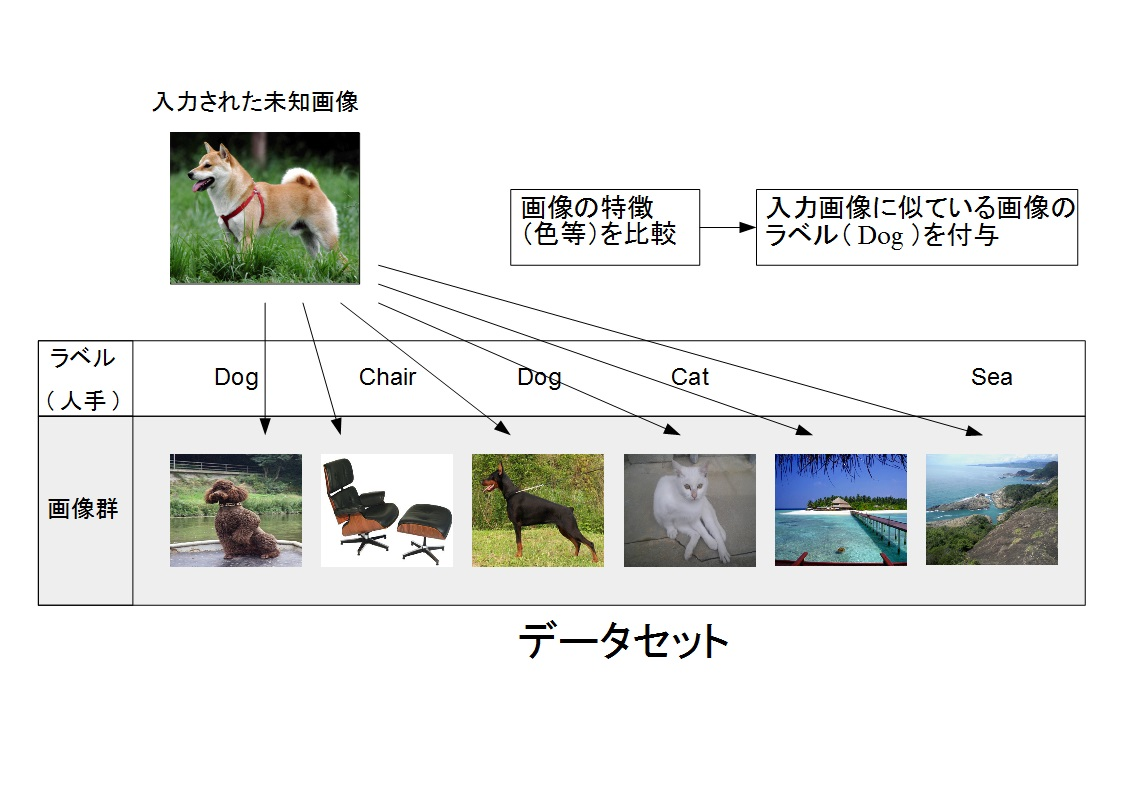
\includegraphics[scale=0.28]{gaiyou.jpg}
 \end{center}
 \caption{一般的な画像アノテーション手法の概要}
 \label{fig:abst}
\end{figure}

まず第一段階として,画像を収集して
各画像にラベルまたはタグと呼ばれる画像の内容を表すテキストを付与する.
このラベルは人間が手動で記述する場合もあるが,
Web上の周辺テキストを伴った画像を使うことで自動推定する場合もある.
それらラベルを付けた画像の特徴を統計的に分析することで,ラベルの持つ特徴を学習する.
次に第二段階として,未知の画像を入力し,その画像特徴と類似する画像群が共通して持つラベルを見つけ,
入力画像にそのラベルを付与する.
この様にして入力された画像の内容を推測するのが自動画像アノテーションである.

% 本稿では,画像の選別手法に工夫をこらし,入力画像に対するラベル付与の精度を高めるための実験を行った.
自動画像アノテーションの分野における研究課題としては,
画像の収集や画像へのラベル付与を自動化することで,
大規模な画像データセットの構築にかかる時間と労力を減らすことがある.
%\subsection{画像アノテーション}
%
%前節で
%ラベル付与の自動化・高精度化の手法が研究されていると述べた.
それらの研究の中でも近年頻繁に研究されているものが,画像のブロブ化である
\cite{duygulu,jeon}.
ブロブ化は各画像を複数の領域に分割し,隣接する領域との特徴の差異を見ることで画像全体を分解することで行う.
これによって得られたブロブ(画像内の物体の塊)は,画像に写っている物体ごとに分割されている可能性が高いので,
注目しているブロブ以外にある物体の有無に左右されることなく,そのブロブに対する精確なラベル付与が可能となる.
このブロブ化をデータセット内の全ての画像に施すことで,高精度の自動画像アノテーションを実現する.

Duygulu\cite{duygulu}らやJeon\cite{jeon}らは,すべての画像はブロブに単語を割り当てることで
内容物を記述することができるという前提で研究を行った.
JeonはDuyguluらの研究を元に,まずブロブと単語の同時分布を学習するためにCMRM(Cross-Media Relevance Model)を開発し,
更にそのモデルを改良した三つのモデルを開発した.
これらは画像を収集する際に自動画像アノテーションを行う確率的生成モデルである.
その結果,Duyguluらが論文で公開した確率的生成モデルの画像アノテーションの平均精度0.20に比べ,
ほぼ倍の0.41という平均精度を示し,再現率についてもはるかによい結果となった.

またこれらの研究とは別のアプローチで自動画像アノテーションの精度向上を目指した研究がある.
渡邉ら\cite{watanabe}は,大規模Web画像データベースと
類似画像検索技術を用いた自動画像アノテーションシステムを実装した.
このシステムは,与えられた画像をクエリとして類似画像検索を行い,
検索結果の画像に付随するテキスト中の単語を確率的指標により評価することで,
特別な事前学習なしに画像を意味付けるキーワードを推定する.
このシステムを用いて5カテゴリ30概念の画像に対するアノテーションを行った結果,
10位内正解率がカテゴリ平均で43~75\%,全概念の平均で約59.1\%であった.

\subsection{テキスト処理}

Web上の画像の周辺テキストから画像の内容を推定するのが自動画像アノテーションであるとみなすこともできる.
このような自動画像アノテーションの研究は多く存在する.
しかしテキスト処理として英語のテキスト処理を行うものが大部分である.
本研究では日本語テキスト処理を使った画像アノテーション手法を提案する.
%
ここでは
自動画像アノテーションを行うために
英語のテキスト処理と日本語のテキスト処理でどのような差があるのか
関連研究から推測する.

テキストの中の特定の対象を選別する問題の参考としてposタガーを考える.
ある研究では英語のposタガーの性能として約8割程度の精度が報告されている\cite{BirdKleinLoper09}.
%,Ibanez:2011:EPS:1964799.1964819
%日本語のposタガーの性能は約9割程度の精度であることが報告されている\cite{UniDicJp2010}.
%この結果はベンチマークや学習データの違いによって変わることがあるため単純に比較することはできないが,
またある研究では日本語のposタガーの性能として約9割程度の精度が報告されている\cite{UniDicJp2010}.
この結果はベンチマークや学習データの違いによって変わるため単純に比較することはできないが,
日本語テキスト処理の方が英語テキスト処理よりも精度が高い可能性を示している.
このことから同じ画像が対象であっても周辺テキストが日本語の場合は,周辺テキストが英語の場合よりも高い精度で
自動画像アノテーションを実現できる可能性がある.
posタガーは単語の並んだ順番を処理する技法でもある.
このことから日本語の適当な手がかり表現を利用する手法は特に高い精度を達成できる可能性がある.

渡邉ら\cite{watanabe}の英語周辺テキストを利用した画像アノテーションの研究では,単純に単語の出現頻度を利用していた.
本研究では日本語の手がかり表現を利用した選別を行う.

\section{提案手法}
\label{sec:way}

%\subsection{概要}
ここでは本研究で提案する自動画像アノテーション手法を説明する.
図\ref{fig:way}に提案手法の概要を示す.
%
\begin{figure}[tb]
 \begin{center}
  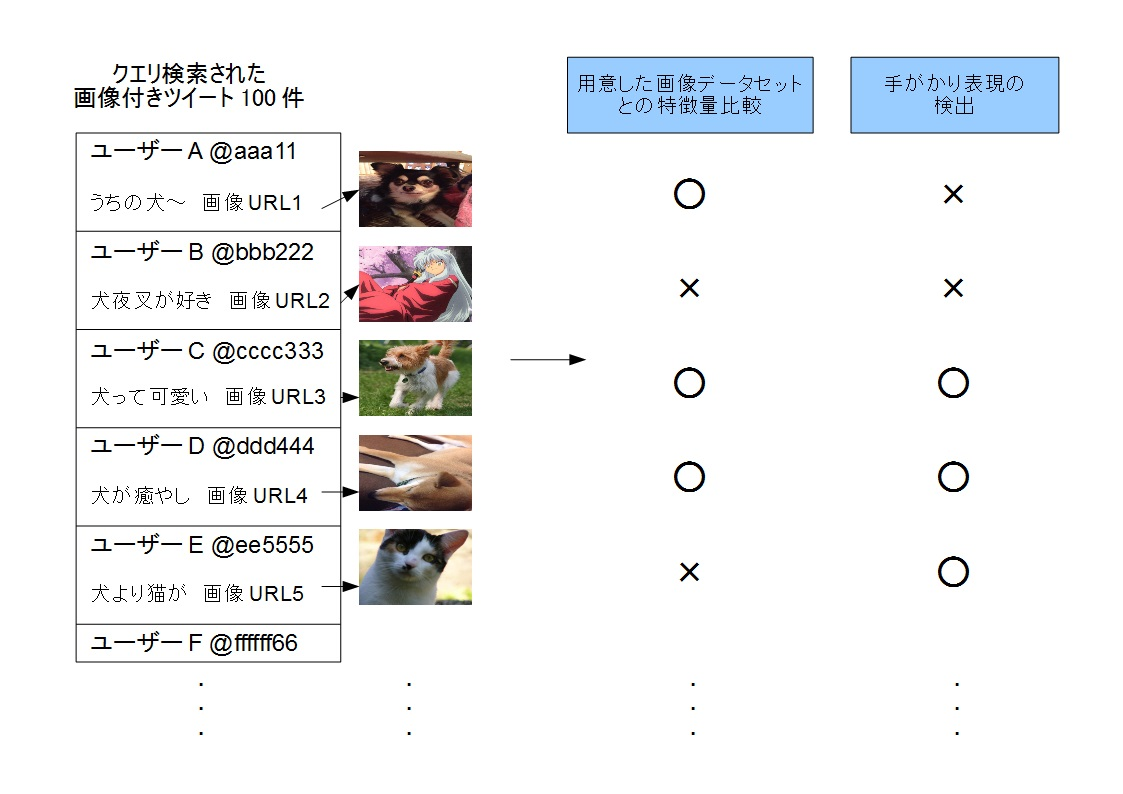
\includegraphics[scale=0.29]{way.jpg}
 \end{center}
 \caption{提案手法の概要}
 \label{fig:way}
\end{figure}
%
提案手法は,ツイート収集,類似画像検索,テキスト検索の3段階で構成される.


%Webから得られた画像と周辺テキストを収集する前処理と,
%類似画像検索とテキスト検索を用いて得られた画像を選別する処理に分けられる.

最初のツイート収集処理においては,Twitter APIを利用し,認識したい物体名をクエリに指定して検索を行い,得られたツイートを収集する.
収集したツイートに付随するURLから,Twitterの公式アップローダにアップロードされた画像を取得する.

次の類似画像検索処理においては,まずユーザが手作業でクエリとして選んだ物体を表す参考画像を一枚,事前に用意する.
参考画像とは,クエリを正しく表していると著者が判断した画像であり,類似画像検索の比較元とする画像である.
この参考画像をクエリとして,収集した画像群から類似画像を選別する.
ここで類似画像とは,クエリとした画像と色の特徴が近い画像のことである.
本研究では参考画像の色ヒストグラム分布と類似した色ヒストグラム分布を持つ画像を類似画像とした.
この結果,参考画像と見た目の類似した画像が選別される.
%%%
%参考画像の選別は人手で行う必要があるが,ImageNetを使って自動化することも出来る.
%しかしこの自動化の処理の実装は今後の課題である.

次のテキスト検索処理においては,選別された画像のツイート本文に
手がかり表現を用いてさらに選別する.
この手がかり表現とは,選別された画像に付随するテキストが何を表しているかの手がかりとなる表現のことである.
ツイート本文中からその表現を検索することで,
そのツイートに付随する画像がクエリを表現しているか否かを判定する.

本研究では,この三つの処理を順次行うことで自動画像アノテーションを実現する.
類似画像検索処理とテキスト検索処理では異なる選別結果が与えられる.
この異なる選別結果の両方で正解と選別された結果を正解とする.
すなわち類似画像検索処理結果とテキスト検索処理結果の積集合を提案手法は出力する.
%%%
%どちらか片方の処理で正解と選別された結果を正解とする論理和処理の結果が提案手法である.
以下では,ツイート収集と,類似画像検索,テキスト検索について詳細に説明する.

\subsection{ツイート収集}
\label{sec:tweetCollect}
Twitter API 1.1の機能を使い,検索したい画像の名称をクエリとし,ツイートを検索する.
この際,オプションとして
%“ -RT filter:images”
``\verb| -RT filter:images|''
をクエリに含める.
%“-RT”
``\verb|-RT|''
は重複したツイートを取得することを避けるために追加した.
%“filter:images”
``\verb|filter:images|''
はTwitterの公式アップローダにアップロードされた画像のみを参照するために使用した.

次に収集した各ツイートから最後尾にあるURL部分を抜き出し,URL先からHTMLソースを入手する.
このHTMLソースから,正規表現でTwitterの公式アップローダに格納されている画像URLを抜き出し,
画像データをコピーして保存することで画像群を収集する.
この処理の際,ツイートしたユーザーがツイートへのアクセス制限を課したり,
ツイートを消去したりすることによって,
収集したツイートのページや画像が格納されているアップローダのURLにアクセスできない場合がある.
このような場合これらのツイートは無視し,画像が正常に保存できたツイートのみを収集する.
%改めてデータベースに格納する.
これらの処理によって,収集したツイートと,ツイートに対応した画像のセットが作成できる.


\subsection{類似画像検索}
\label{sec:similar}

%%%色ヒストグラムは大学生向けの教科書に載っている話題なので本来なら詳細に説明する必要はありません.
%%%何か説明する必要があるのは色ヒストグラムについて何か特別な工夫を提案している場合のみです
提案手法では,各色が画像中に何ピクセルあるかを数えた色ヒストグラムの分布を画像の特徴量として扱い,
この分布が参考画像と類似している画像を類似画像として選別する\cite{Datta08imageretrieval:}.
色ヒストグラム処理は
%,ブログ「人工知能に関する断創録」
%\footnote{人工知能に関する断創録, http:\slash\slash{}aidiary.hatenablog.com}
\url{http://aidiary.hatenablog.com}
で公開されているプログラムを参考に実装した.

色ヒストグラムはRGBの3色8ビットをそのままで計算すると16,777,216次元ベクトルとなり
計算にかかる時間が非常に大きくなる.
提案手法ではRGBの各色を4段階の色の濃さに減色して64色に減色した上でヒストグラムを算出する.
具体的にはRGBの各3色の色の濃さの組み合わせ$(256)^3=(2^8)^3$色を0から3の4段階に減色した$64=4^3$色についての色ヒストグラムを使う.
%各番号は分けられた
例として
64色に減色した画像と,
その色ヒストグラムの棒グラフを
図\ref{fig:color}に示す.
%
\begin{figure}[tb]
 \begin{center}
  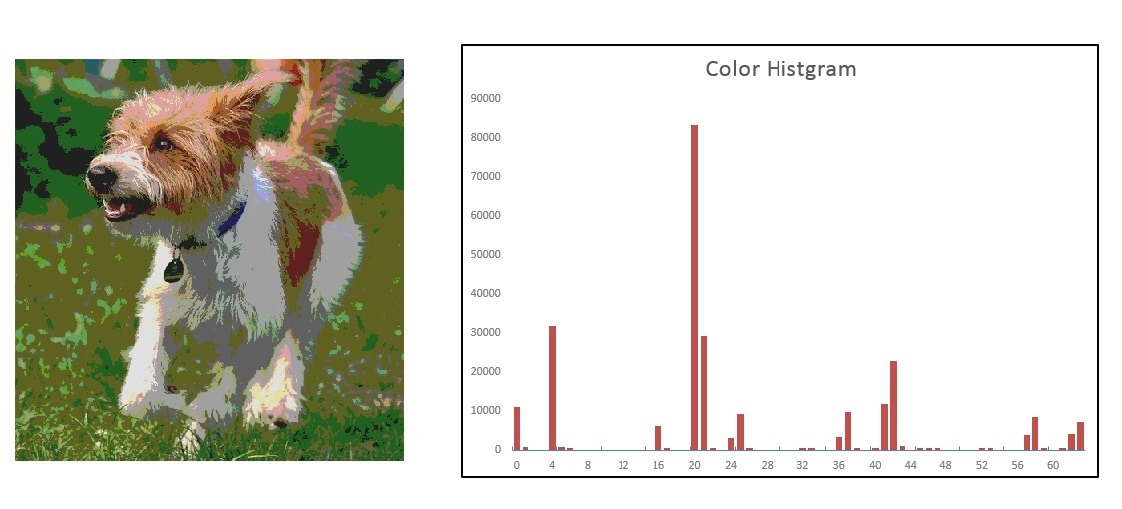
\includegraphics[scale=0.28]{colorhist.jpg}
 \end{center}
 \caption{色ヒストグラムの例}
 \label{fig:color}
\end{figure}
%
%
%OpenCVの色ヒストグラム類似度計測関数のドキュメントに色ヒストグラムを使う手法の詳細や参考文献が書いてあったはずなので色ヒストグラム処理の話を追加してください
図\ref{fig:color}左の犬の画像はRGB値がそれぞれ4通りしかないことから,
三色の色の組み合わせ総数は64であるため,棒グラフの横軸は0から63となっている.
横軸のビンの値は以下の式で表される.
\begin{eqnarray}
\mbox{bin} = (16 * R) + (4 * B) + (1 * G)
\end{eqnarray}
このときR,G,Bの値はそれぞれの色番号である.
例えば
図\ref{fig:color}右の棒グラフで
大きい値をとっているbin=20は(R,G,B)=(1,1,0)であり,
画像中で濃い黄緑が
広い面積をとっていることがわかる.

本手法では,取得した画像群から
参考画像と類似した画像を選別する.
そのため,クエリを正しく表している
参考画像を事前に人手で選別しておかなければならない.
この処理はImageNetを使って自動化することも出来るが
ImageNetの選別カテゴリにない対象も多くある.
例えば犬の画像はImageNetから自動で収集できるが,
%\ref{sec:experiment}
4
節の実験でクエリ対象とした柴犬のカテゴリはImageNetには存在しない.
この様な場合もあるため本実装では参考画像の選別は手動処理としている.
%
選別された参考画像と収集した画像群は全て同じ320$\times$240サイズのJPEG形式に変換する.
これは色ヒストグラムを算出する際に,全ての画像において画素の記述方法を統一するためである.
次に,\ref{sec:tweetCollect}節で収集した画像と参考画像を減色した画像の色ヒストグラムを算出する.
%それぞれのデータを作成する.

次に参考画像のヒストグラムデータをクエリとして,
Histogram Intersubsection\cite{Swain91colorindexing}
の考え方を使って
類似度を算出する.
Histogram Intersubsectionとは
二つの色ヒストグラム
$H_1,H_2$
が与えられたときの類似度を
以下の式で与える手法である.
%
\begin{eqnarray}
\mbox{Similarity} = \frac{\sum_{i=0}^{63} \min(H_1[i],H_2[i])}{\sum_{i=0}^{63} H_1[i]}
\end{eqnarray}
%
ここで$H_k$は$k$番目の画像の色ヒストグラムであり,
$H_k[i]$はそのヒストグラムの$i$番目のビンの値である.
%このとき2つのヒストグラムをH1,H2,ヒストグラムHのi番目のビンの値をH[i]と定義する.
なお,$H_1$は参考画像のヒストグラムである.
この類似度は正規化がされているため,値は0.0から1.0となり,
二つのヒストグラムが似ているほど大きな値をとる.
この類似度が設定した閾値を超えた画像を,クエリを表している画像として選別する.
%閾値の設定方法については後述する.
%%%%%%%%%%閾値が明確に決められない場合にROCカーブを描いて性能を比較する場合も%%%%%%%%%%%%
%%閾値を 0 から1まで 0.01 ずつ大きくしていき,それぞれの閾値において類似画像検索の適合率と再現率を求める.%%
\subsection{テキスト検索}
\label{sec:textSearch}

本研究の目的はWebからの画像収集の自動化である.
Webには周辺テキストを伴った画像は大量に存在する.
よって,選別対象の母数はいくらでも大きくすることができるため本研究では再現率は重視しない.
高い適合率を目標とする.

\subsubsection{予備実験}
\label{sec:yobijikken}

予備実験として
\ref{sec:tweetCollect}節で説明した方法で収集したツイート集合から
犬と猫の画像を収集する実験を行った.
単純な手がかり表現として
“本物”,“写真”,“いる”,“撮”のいずれかの文字列と“犬”または“猫”の文字を含むツイートを選別した.
この単純なテキスト選別の方法では,3割しか正解画像を含んでいないデータセットしか得る事はできなかった.
しかし犬全般ではなく柴犬を検索したところ,4割以上とやや高い適合率を得ることができた.
猫全般と,猫の品種であるシャム猫,メインクーンについても同様の傾向がみられた.
そこで本研究では犬全般の様な広いカテゴリではなく柴犬の様な狭いカテゴリを検索対象にする.
%犬全般をクエリとしたい場合は
%柴犬,シープドック,プードルなどの狭いカテゴリについての検索結果を合算することとする.
%この様なサブカテゴリはWordNetを使うことで得ることができる.

% この狭いカテゴリのみを扱う場合に適合率を向上させるために,
% 手がかり表現をさらに増やす方法を...

%そのための手がかり表現を次の方法で収集した.
%\ref{sec:tweetCollect}節で
%収集したツイートの本文から手がかり表現を見つけ,そのツイートの持つ画像を選別する.

\subsubsection{手がかり表現の収集とその利用方法}

次に手がかり表現をさらに増やすことで
%\ref{sec:yobijikken}節で使った手がかり表現よりも
適合率を上げられないか検討する.
手がかり表現は,次の方法で収集する.
%
%\ref{sec:tweetCollect}節の手法で犬,狐,猫のツイートを収集する.
%これらの広いカテゴリの検索対象は提案手法では扱わないこととしている点に注意する.
\ref{sec:tweetCollect}節の手法で収集した犬,狐,猫のツイートの中で正解画像を含むツイートのみを人手で選別する.
そして選別したツイートに含まれる出現頻度の高い動詞,形容詞のみを選別する.
選別した動詞と形容詞の一部を
表\ref{tab:predicate}に示す.
収集したツイート100件からは,動詞が73,形容詞が46抽出できた.
これらの単語を
1ツイート中に合計三つ以上含んでいるツイートを選別するのが提案手法である.
なお,
%\ref{sec:experiment}
4節で行う本手法の評価実験では,この手がかり表現の収集に利用したツイートは除外している.
またこの三つという数は,抽出に使用したツイート1文から抽出できた動詞,形容詞の数の平均を採用した.
品詞の選別にはMeCabバージョン0.996
\footnote{MeCab, http:\slash\slash{}mecab.googlecode.com\slash{}svn\slash{}trunk\slash{}mecab\slash{}doc\slash{}index.html}
を利用した.


% 本手法で使用する手がかり表現は以下の手順で得る.
% まずTwitterから収集した画像付きツイートから,正しく画像の内容に言及しているツイートのみを人手で選別する.
% 選別したツイート群を言語処理にかけ,それぞれのツイートから動詞と形容詞を抽出する.
% 抽出した単語から重複をなくした集合を手がかり表現の集合とみなし,画像選別に用いる.
% なお,本手法で使用した手がかり表現の集合を得るために使用したツイートは,
% \ref{sec:examination}節で使用した複数のカテゴリのツイートを収集した際,
% 評価実験に使用しなかった一部のツイートから選別した合計100件のツイートである.
% また言語処理には形態素解析エンジンMecab
% (\url{http://mecab.googlecode.com/svn/trunk/mecab/doc/index.html})のver0.996を使用し,
% ツイート中から分割された単語のうち品詞が動詞と形容詞のもののみを抽出したものを使用している.

% 抽出した手がかり表現の一部を表\ref{tab:predicate}に示す.

\begin{table}[bt]
\begin{center}
\caption{抽出された手がかり表現の例}
\label{tab:predicate}
\begin{tabular}{|l|l|}\hline
動詞& 撮っ,佇む,持っ,する,たつ,吠え,飼い \\ \hline
形容詞& かわいい,よい,近かっ,ほしい,可愛い \\ \hline
\end{tabular}
\end{center}
\end{table}

% \subsubsection{ツイート文の解析}

% 収集したツイートを1文ずつMecabにかけ,
% 手がかり表現の集合に含まれる単語がそのままの形でツイート文に含まれているか1つずつ調べ,
% 1ツイート中に合計三つ以上の単語を含んでいるツイートの持つ画像は,
% クエリとして選んだ物体を表していると判断した.
% この3という数は,抽出に使用したツイート1文から抽出できた動詞,形容詞の数の平均を採用した.

\section{評価実験}
\label{sec:experiment}

ここでは提案手法に適していると考える狭いカテゴリの具体例として柴犬とシャム猫の画像の収集実験を行う.
広いカテゴリである犬一般や猫一般の画像の収集については
%\ref{sec:examination}
5節で考察する.

\subsection{データセット}

%評価実験として提案手法で柴犬の画像を選別する実験を行い,選別結果の精度評価を行った.
%%本稿では,Twitterに投稿された画像付きツイートを収集し,データとして用いた.

柴犬の画像収集は以下のように行った.
類似画像検索の入力に使用する参考画像としてWikipedia\footnote{Wikipedia, http://ja.wikipedia.org/}内の柴犬の記事にある画像を使用した.
ツイートの収集は2015年1月27日に,柴犬をクエリとして
\ref{sec:tweetCollect}節で説明したようにツイートを収集した.
その結果として得られた3,462件のツイートと画像を収集した.
%これらのツイートと画像に参考画像を加えたものをデータセットとする.
このデータ群を提案手法でアノテーションすることで得られる最終的な選別結果の画像に,
どれだけ柴犬の画像が含まれているかを人手で評価し,適合率を算出した.
%適合率は類似画像検索の選別結果に含まれる正解データの割合である.

同様にシャム猫の画像収集も行った.
Wikipedia内のシャム (ネコ)の記事にある画像を参考画像として,
シャム猫をクエリとして得られた932件のツイートと画像を提案手法で選別し,
その選別結果の精度評価を行った.
%これらのツイートと画像をデータセットとした.

\subsection{実験結果}
\label{sec:expresult}

収集された画像群に対し類似画像検索とテキスト検索の両方で選別を行う提案手法を適用した.
適用した結果と,
画像群を人手で選別した正解データとの比較結果を
%本手法による結果を人手で選別し,画像選別精度を評価した
表\ref{tab:result-shiba}に示す.
なお“柴犬”と“シャム猫”は検索クエリに指定したカテゴリ名であり,取得数はクエリによって得られたツイートの数である.
また選別数は提案手法が各カテゴリの正解画像とみなした画像の数であり,
正解数は提案手法が出力した画像を人が実際に見て正解と判断できた画像の数である.

%まずデータセットの柴犬の画像3462枚とシャム猫の画像932枚に対し,
%各画像の色ヒストグラムデータを作成し,参考画像と比較して類似度を算出する.
%求めた類似度が設定した閾値を上回る画像を,クエリを表している画像として選別する.
%このとき閾値を0.58とした.
類似画像検索の処理で必要となる閾値は0.58とした.
この閾値は犬,猫,狐,海,椅子の画像各20枚に対して同様の実験を行い,そこで適合率が最大となるような閾値を決定した.
類似画像検索で柴犬の画像であると判断した画像は1,338枚,シャム猫の画像であると判断した画像は430枚であった.

さらに選別した画像に対応するツイート文に対して
\ref{sec:textSearch}
節で説明したテキスト検索処理を行い,
条件を満たしたツイートに付随する画像を柴犬を表している画像として選別した.
この結果,柴犬の画像であると判断された画像は429枚,シャム猫の画像であると判断された画像は159枚となった.

%\subsection{評価}

柴犬をクエリとして提案手法が出力した429枚の画像のうち,人手で柴犬を表していると判断できる画像は336枚であった.
シャム猫をクエリとして提案手法が出力した159枚の画像のうち,人手でシャム猫を表していると判断できる画像は132枚であった.
この結果から適合率を求めると,
提案手法によって得られた画像セットの適合率はそれぞれ約0.78,約0.83であり,
含まれる誤りの画像は2割程度であると判断できる.

%これは\ref{sec:rel-image}節で述べた許容範囲内である3割を下回っており,
%画像認識アルゴリズムのトレーニングセットとして十分に機能するといえる.

\begin{table}[tb]
\begin{center}
\caption{提案手法による柴犬とシャム猫の画像の選別の精度}
\label{tab:result-shiba}
\begin{tabular}{|l|r|r|r|r|}\hline
カテゴリ名& 取得数& 選別数& 正解数& 適合率(\%) \\ \hline \hline

柴犬& 3462& 429& 336& 0.78 \\ \hline
シャム猫& 932& 159& 132& 0.83 \\ \hline
\end{tabular}
\end{center}
\end{table}

\section{考察}
\label{sec:examination}

%本研究ではTwitterからの画像の収集方法について議論した.
本研究ではTwitterから画像を収集した.
一般的に一つのツイートに含まれる文は多くて3文程度である.
そのため係り受け解析によって詳細にツイート文に含まれる単語の前後の文節を解析することをしなくても,
単純に単語の共起関係を見るだけで文節の内容を推測できる.
ブログのような長い文節が対象の場合には係り受け解析が必要となると推測される.
または長い文節ならば含まれる単語数も増えるため,単語の出現頻度のヒストグラムから内容を推測することもできる.
しかし単語の共起関係だけでおおよその内容が推測できるのはツイッターの特性である.
その反面Twitterでの検索結果には説明が困難な偏りが見られた.
具体的には犬,猫,狐などの画像をテキスト検索のみで探そうとすると非常に多くの関係ない画像が出現した.
この原因などについてここでは考察する.


%\ref{sec:expresult}節で述べたように,
%柴犬をクエリにして得られた画像3462枚を提案手法で選別した結果,得られた画像数は429件となった.
%しかし本手法の各手順で,柴犬を表しているのに柴犬の画像ではないと判断されてしまった画像もある.
%この節では提案手法のうち2つの選別処理やその組み合わせが適切かどうか考察する.

%\subsection{考察実験}
\subsection{データセット}

提案手法では犬,猫,狐のような広いカテゴリは検索の対象としなかったが,
これらを検索対象とした場合の性能を示したのが
表\ref{tab:result-ex}である.

表\ref{tab:result-ex}の実験に使用した
データの収集は2015年1月27日に,“[カテゴリ名] -RT filter:images”をクエリとして
ツイートを収集し,
収集したツイート中から無作為にそれぞれ300件ずつツイートを選び,対応する画像を取得した.
ただしここで[カテゴリ名]は犬,猫,狐,椅子,メインクーンの五つである.
またメインクーンについてはクエリを含むツイートが少なく,
192件しか取れなかった.
%犬,猫,狐はある程度大きなカテゴリの中で,Twitterに画像がありそうなものを選んだ.
%椅子は動物以外での選別精度を確かめるために選んだ.
%メインクーンは評価実験に使用した柴犬やシャム猫と同程度の広さのカテゴリの結果を知るために選んだ.
%
%取得できたツイートと画像に参考画像を加えたものを,各カテゴリのデータセットとする.
こうして収集した画像を人手で選別した結果と提案手法で選別した結果を比較した.
%ておき,各選別手法でどれだけの適合率で画像を選別できたかを評価する.
人手での選別の際,クエリが動物であればその動物の顔が半分以上見えていれば正解とした.
クエリが椅子の場合は,人や物などの障害物が画像中に写っている場合であっても
椅子のほぼ全体が画像内に収まっていれば正解とした.

表\ref{tab:result-ex}では,収集した最大300枚の画像またはツイートを対象に,
類似画像検索のみを使用した場合を(1),
テキスト検索のみを使用した場合を(2)としている.
% ,類似画像検索とテキスト検索の和(1∪2),
% 提案手法である類似画像検索とテキスト検索の積(1∩2)の選別の4手法である.
% 表\ref{tab:result-ex}において
(1 $\cup$ 2)
は類似画像検索の選別結果とテキスト検索の選別結果の和集合を選別結果として扱う場合を表す.
(1 $\cap$ 2)
は類似画像検索の選別結果とテキスト検索の選別結果の積集合を選別結果として扱う場合を表す.

%実験結果の再現率,適合率,F 値をまとめたものを表\ref{tab:result-ex}に示す.
ここで,再現率は人手で判定したクエリを表す画像のうち実際に選別できていた正解データ画像の割合である.
さらに,求めた再現率および適合率から F 値を算出する.
F 値($F\verb|-|measure$)は適合率($precision$)と再現率($recall$)の調和平均であり,次式で求める.

\begin{eqnarray}
F\verb|-|measure = \frac{2・precision・recall}{precision+recall}
\end{eqnarray}

\subsection{各カテゴリの選別結果の特徴}
%\subsection{偏りの効果}

Twitterにおいて,ツイートと画像のある種のミスマッチの影響が特に顕著に見られたのが狐についての結果である.
狐で得られた画像を人手で選別した結果,300枚中7枚しか正解がなかった.
狐のカテゴリでは収集した画像に狐が写っている画像が極端に少なく,
その選別結果の評価は困難であった.
これは狐が身近にいる動物ではないため,写真が少なく,
代わりにイラストが多く含まれていたことが理由としてあげられる.
また,
%これは狐という単語には動物として狐以外の様々な意味を内包している事が原因ではないかと考えられる.
%例えば
ブラウザのFirefoxを“狐”と表現する場合などがあり,この画像もノイズとなった.

犬と猫に対しても狐ほどではないが類似したミスマッチが見られた.
クエリ“犬”で得られた画像を人手で選別した結果は,300枚中130枚が正解となった.
クエリ“猫”で得られた画像を人手で選別した結果は,300枚中105枚が正解となった.
検索対象を直接表す単語をTwitterの検索APIに入力しているにも関わらず2/3が目的外の画像であった.
しかし類似画像検索を使って間違った画像を除外することで,適合率は約6割を達成できている.
テキスト検索はあまり効果をあげておらず適合率は4割程度である.
しかし類似画像検索とテキスト検索の結果の積集合をとると7割程度の適合率を実現している.
これは場合によっては広いカテゴリを対象としたクエリも利用できる可能性があることを示唆している.
ただしこのときの再現率は3割以下であり収集できた画像は30枚以下であった.
%これはクエリの種類によっては数枚しか画像が収集できない可能性を示しており,
%サブカテゴリでの検索の方が安全であることが推測される.

メインクーンは猫の一種である.
これをクエリとして得られた画像を人手で選別した結果は,192枚中142枚が正解と判別できた.
過半数が対象の画像であり,より狭いサブカテゴリでの検索は高い適合率を達成できることを示している.
特に類似画像検索とテキスト検索の結果の積集合の結果は選別した全ての画像が正解となっている.
しかし類似画像検索の再現率は1割となっている.
メインクーンの収集画像を見ると
毛色や撮る状況によって,色の分布が他の動物より大きく変動している様子がみられた.
これが類似画像検索の再現率を下げていると考えられる.


クエリ“椅子”で得られた画像を人手で選別した結果は,300枚中149枚が正解と判別できた.
椅子の選別結果は,全体的に犬より悪い結果となっている.
これは,椅子を表すツイートにおいて動詞や形容詞があまり使われておらず,
抽出した手がかり表現の集合にも椅子に適した表現が少なかったことがあげられる.

\begin{table}[tb]
\begin{center}
\caption{各カテゴリの選別における再現率,適合率,F値}
\label{tab:result-ex}
\begin{tabular}{|l|r|r|r|r|}\hline
&& 再現率& 適合率& F値\\ \hline \hline
犬
& 類似画像検索(1)& 0.246& 0.640& 0.356 \\ \cline{2-5}
& テキスト検索(2)& 0.669& 0.446& 0.535 \\ \cline{2-5}
& 和集合(1$\cup$2)& 0.792& 0.464& 0.585 \\ \cline{2-5}
& 積集合(1$\cap$2)& 0.123& 0.696& 0.209 \\ \hline
猫
& 類似画像検索(1)& 0.371& 0.582& 0.453 \\ \cline{2-5}
& テキスト検索(2)& 0.610& 0.372& 0.462 \\ \cline{2-5}
& 和集合(1$\cup$2)& 0.705& 0.372& 0.487 \\ \cline{2-5}
& 積集合(1$\cap$2)& 0.276& 0.725& 0.400 \\ \hline
狐
& 類似画像検索(1)& 0.571& 0.095& 0.163 \\ \cline{2-5}
& テキスト検索(2)& 0.429& 0.016& 0.031 \\ \cline{2-5}
& 和集合(1$\cup$2)& 0.571& 0.020& 0.039 \\ \cline{2-5}
& 積集合(1$\cap$2)& 0.429& 0.100& 0.162 \\ \hline
椅子
& 類似画像検索(1)& 0.309& 0.500& 0.382 \\ \cline{2-5}
& テキスト検索(2)& 0.497& 0.411& 0.450 \\ \cline{2-5}
& 和集合(1$\cup$2)& 0.678& 0.479& 0.561 \\ \cline{2-5}
& 積集合(1$\cap$2)& 0.128& 0.613& 0.211 \\ \hline
メインクーン
& 類似画像検索(1)& 0.106& 0.882& 0.189 \\ \cline{2-5}
& テキスト検索(2)& 0.606& 0.775& 0.680 \\ \cline{2-5}
& 和集合(1$\cup$2)& 0.648& 0.773& 0.705 \\ \cline{2-5}
& 積集合(1$\cap$2)& 0.063& 1.000& 0.119 \\ \hline
\end{tabular}
\end{center}
\end{table}

\subsection{類似画像検索による画像選別精度評価}
類似画像検索の選別精度は,全体的に再現率が低く,適合率が高い傾向にある.
適合率が高い理由としては,参考画像として人手で確実に正解の画像を選ぶので,
類似画像検索では正解に近い色の分布を持つものが選ばれるからである.
逆に,再現率が低いのは,選別する数が少ないため,
その中に含まれる正解データも必然的に少なくなることが理由である.
設定した閾値が0.58と高めであるため,犬,猫,狐では選別結果の画像数もかなり少なかった.
改良案としては,類似画像検索に使う閾値を選別するカテゴリごとに分けることや,
類似画像検索に使用する特徴量を変えることがあげられる.

\subsection{テキスト検索による画像選別精度評価}

テキスト検索の選別では,基本的に多くの画像をそのカテゴリの画像に選別しており再現率が高い傾向がある.
これは,手がかり表現の集合に基本的な動詞などが含まれているため,
多くのツイートがこの選別条件に当てはまることが理由である.
その結果,全体的に再現率が高く適合率が少し低めとなっている.
しかし猫,犬,椅子を選別した結果のF値は0.5程度であり,
改良の余地はまだ大きい.

\subsection{2手法の組み合わせによる画像選別精度評価}
類似画像検索とテキスト検索,2手法の検索結果の和集合(1$\cup$2)では,
狐以外の全カテゴリにおいていずれか一つの手法による選別結果よりF値が高くなっている.
これは,選別される画像の割合が増えた以上に,その結果に含まれる正解データの割合が増えたためである.
反面,選別結果には多くの間違いも含まれており,
%画像認識のトレーニングセットとして使えるまでには至っていない.
目標とする適合率には届いていない.

しかし,2手法の結果の積集合(1$\cap$2)ではF値が極端に低く,
各カテゴリの画像に選別される画像自体が少ない.
その代わりにその中に含まれる正解データの割合は非常に高くなっている.
犬や猫は7割近い適合率となり,椅子の結果でも6割の適合率となっている.
これらのことから,現状の2手法の組み合わせとしては積集合が有用であることがわかる.
しかし,選別の結果得られた画像はかなり少ない.

2手法の結果の積集合を出力する提案手法では多くのツイートを取得できた場合は,
画像認識アルゴリズムのトレーニングセットとして利用可能な画像枚数となったが,
狐などでは十分な画像が得られない可能性が高い.
%しかし,本研究の目的のような狭い範囲のカテゴリにおける画像選別には,
%提案手法にも収集作業を繰り返すことである程度利用できることがわかる.

\section{まとめ}
\label{sec:format}
本稿では,類似画像検索とテキスト検索を用いた自動画像アノテーション手法を提案し,
自動画像アノテーションにおける日本語ツイートの有用性を実験により確認した.
本手法は,Twitterから画像付きツイートを収集し,
画像特徴量を用いた類似画像検索と手がかり表現を用いたテキスト検索を併用し,
収集された画像がクエリで指定した物体を表しているかどうかを判別するものである.
提案する自動画像アノテーション手法では収集された画像が
画像認識アルゴリズムの学習画像として利用可能となるように適合率を重視した.
本手法はクエリ対象として犬や猫といった広いカテゴリの場合よりも,
柴犬やシャム猫といった狭いカテゴリを対象とした場合に,高い適合率を示すがわかった.

%\vspace{30mm} <- 文献が本文と近すぎるときは適宜利用してください.
\vspace{2em}

%\begin{thebibliography}{99}
\bibliographystyle{ipsjunsrt}
\bibliography{fujii}
%\end{thebibliography}

\end{document}
